% Taken from:
% http://steventhornton.ca/blog/markov-chains-in-latex.html
\documentclass{standalone}

\usepackage{tikz}
\usetikzlibrary{automata, positioning}
\begin{document}
    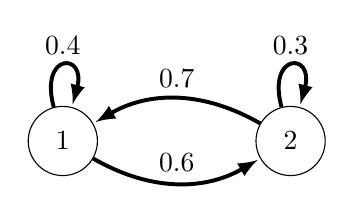
\begin{tikzpicture}

        % Add the states
        \node[state,
            text=black,
            draw=black,
            fill=white] (s_1) {$1$};
        \node[state,
            right=2cm of s_1,
            text=black,
            draw=black,
            fill=white] (s_2) {$2$};

        % Connect the states with arrows
        \draw[every loop,
            auto=right,
            line width=0.5mm,
            >=latex,
            draw=black,
            fill=black]
            (s_1) edge[bend right, auto=left]  node {$0.6$} (s_2)
            (s_2) edge[bend right, auto=right] node {$0.7$} (s_1)
            (s_1) edge[loop above]             node {$0.4$} (s_1)
            (s_2) edge[loop above]             node {$0.3$} (s_2);
\end{tikzpicture}
\end{document}
